\documentclass{article}%
\usepackage[T1]{fontenc}%
\usepackage[utf8]{inputenc}%
\usepackage{lmodern}%
\usepackage{textcomp}%
\usepackage{lastpage}%
\usepackage[head=40pt,margin=0.5in,bottom=0.6in]{geometry}%
\usepackage{graphicx}%
%
\title{\textbf{Trabajadores de Venalum exigen respeto al contrato colectivo}}%
\author{El Nacional Web}%
\date{30/09/2018}%
%
\begin{document}%
\normalsize%
\maketitle%
\textbf{URL: }%
http://www.el{-}nacional.com/noticias/protestas/trabajadores{-}venalum{-}exigen{-}respeto{-}contrato{-}colectivo\_253768\newline%
%
\textbf{Periodico: }%
EN, %
ID: %
253768, %
Seccion: %
Protestas\newline%
%
\textbf{Palabras Claves: }%
NO\_TIENE\newline%
%
\textbf{Derecho: }%
2.3%
, Otros Derechos: %
NO\_TIENE%
, Sub Derechos: %
2.3.4%
\newline%
%
\textbf{EP: }%
SI\newline%
\newline%
%
\textbf{\textit{Los empleados realizaron una asamblea para denunciar la violación del gobierno a las tablas salariales}}%
\newline%
\newline%
%
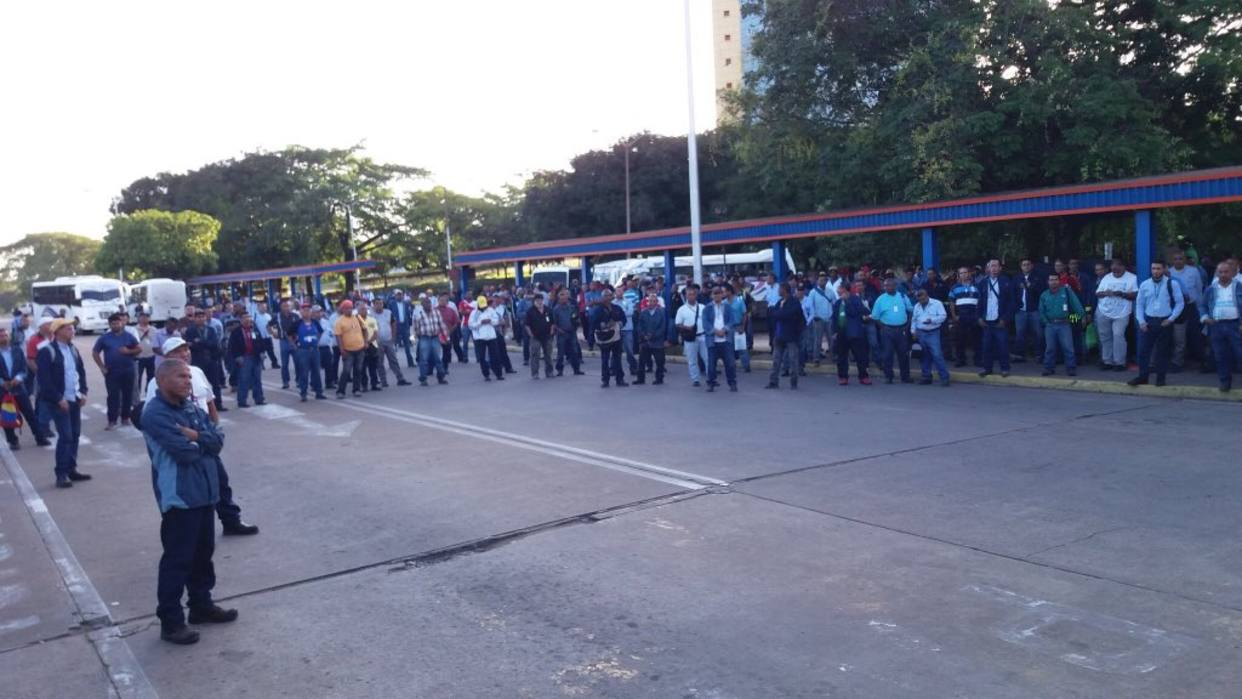
\includegraphics[width=300px]{146.jpg}%
\newline%
%
Trabajadores de la~Industria Venezolana de Aluminio (Venalum) exigen respeto por parte del gobierno al contrato colectivo.%
\newline%
%
Reportes de Twitter indican que los empleados realizaron una asamblea este domingo para denunciar que, tras el pago de la quincena, el gobierno violó también las tablas salariales.%
\newline%
%
Usuarios reportan que los portones de las empresas básicas de Guayana amanecieron cerrados%
\newline%
%
\end{document}